\documentclass[acmtog]{acmart}
\usepackage{graphicx}
\usepackage{subfigure}
\usepackage{natbib}
\usepackage{listings}
\usepackage{bm}

\definecolor{blve}{rgb}{0.3372549 , 0.61176471, 0.83921569}
\definecolor{gr33n}{rgb}{0.29019608, 0.7372549, 0.64705882}
\makeatletter
\lst@InstallKeywords k{class}{classstyle}\slshape{classstyle}{}ld
\makeatother
\lstset{language=C++,
	basicstyle=\ttfamily,
	keywordstyle=\color{blve}\ttfamily,
	stringstyle=\color{red}\ttfamily,
	commentstyle=\color{magenta}\ttfamily,
	morecomment=[l][\color{magenta}]{\#},
	classstyle = \bfseries\color{gr33n}, 
	tabsize=2
}
\lstset{basicstyle=\ttfamily}

% Title portion
\title{Assignment 2:\\ {Geometric Modeling}} 

\author{Name:\quad Yang Hongdi  \\ student number:\ 2019533234
\\email:\quad yanghd@shanghaitech.edu.cn}

% Document starts
\begin{document}
\maketitle

\vspace*{2 ex}

\section{Introduction}
In this project, there is an object consisted of 3 bezier surfaces with L1 continuity. There is also a 
Bspline surface which can be interactively edited by imgui. And Phong lighting by one light is performed.


\section{Implementation Details}
\subsection{Bezier curve evaluation}
For bezier curve evalution, I simply use the iterative method as $$Q(i) = (1-t) P(i) + tP(i+1)$$
and iterative do this until there is only one point left. When there are only two points, the line connects them is the tangent we need, we record it
and use it to calculate the normal later.

\subsection{Bezier surface evaluation}
To construct a Bezier surface, we need control points of two directions and the division num to determine how many points we need to evaluate.
\begin{lstlisting}
class BezierSurface {
 public:
  vector<vector<vec3>> control_points_m_;
  vector<vector<vec3>> control_points_n_;
  int div_num;
  //...member functions
};
\end{lstlisting}
\quad We first evaluate the bezier curves along one direction, then we get the control points and we use it to construct a Bezier curve and evaluate this bezier curve again.
Then we have the point's postion and we record the tangent in this direction.\\
We repeat this procedure again in another direction, the point's postion should be the same and we get another tangent. The cross product of the two tangents will be the
normal of this point.
\begin{lstlisting}
Vertex BezierSurface::evaluate
(vector<vector<vec3>>& control_points,
							float u, float v) {
BezierCurve order1_curve(control_points.size());
for (int i = 0; i < control_points.size(); i++)
{
BezierCurve tempcurve(control_points[i]);
order1_curve.setControlPoint(i, 
	tempcurve.evaluate(v).position);
}
return order1_curve.evaluate(u);                              
}
\end{lstlisting}

\subsection{BezierSurface rendering}
After evaluating enough points on the surface, we can add the points to the vertex array of the object.
For each 2x3 points, we can construct two triangles, like

\begin{lstlisting}
int point_num = div_num + 1;
for (int i = 0;i < point_num - 1; i++)
{
	for (int j = 0; j < point_num - 1; j++)
	{
	new_object.indices.push_back(i * point_num + j + 1);
	new_object.indices.push_back(i * point_num + j);
	new_object.indices.push_back((i+1) * point_num + j);
	///1st triangle

	new_object.indices.push_back(i * point_num + j + 1);
	new_object.indices.push_back((i+1) * point_num + j);
	new_object.indices.push_back((i+1) * point_num + j 
													+ 1);
	///2nd triangle
	}
}
\end{lstlisting}
then we have the vertex array and the indices array, by attaching them to VAO, VBO
we can render the Bezier Surface.
\subsection{Bezier Surface stitching}
For Bezier surface stitching, I simply set their 1st and last control point to be the same postion and make sure the control polygon is colinear.

\subsection{Bspline curve evaluation}
For Bspline curve evaluation, we can use methods similar to Bezier curve. First, we define the degree to be $p$ and $n$ control points, and we need 
to have $m$ knots satisfying $m = n + p + 1$. To make sure we can reach the final control point and first control point, we need to have $p + 1$knots to be 0 and 
$p + 1$ knots to be 1.\\
To evaluate the point, we use the formula
$$Q_i = (1 - a_i)P_{i-1} + aiP_i$$
\\
$$a_i = \frac{t-u_i}{u_{i+p} - u_i} \ \ \ for\ k -p+1 \leq i \leq k$$
k is where $u_k \leq t < u_{k+1}$.\\
For this formula, we can iteratively compute the control points until there is only one  point, and we record the tangent when there are two 
control points(like what we do with Bezier curve), then we can get the position and tangent of the point.

\subsection{Bspline Surface construction and Rendering}
Quite like that with BezierSurface, we evaluate the points from two directions, we get two tangents, and we compute the normal. Then we are able to render it using the
vertex array and indices array.

\subsection{Interactive Editing}
I use the dear imgui library to edit. inclue the header files.
\begin{lstlisting}
#include "imgui.h"
#include "imgui_impl_glfw.h"
#include "imgui_impl_opengl3.h"
\end{lstlisting}
for each control point, we can change its position and then evaluate the points again.
\section{Results}
\begin{figure}[h]
	\begin{minipage}[b]{.4\linewidth}
		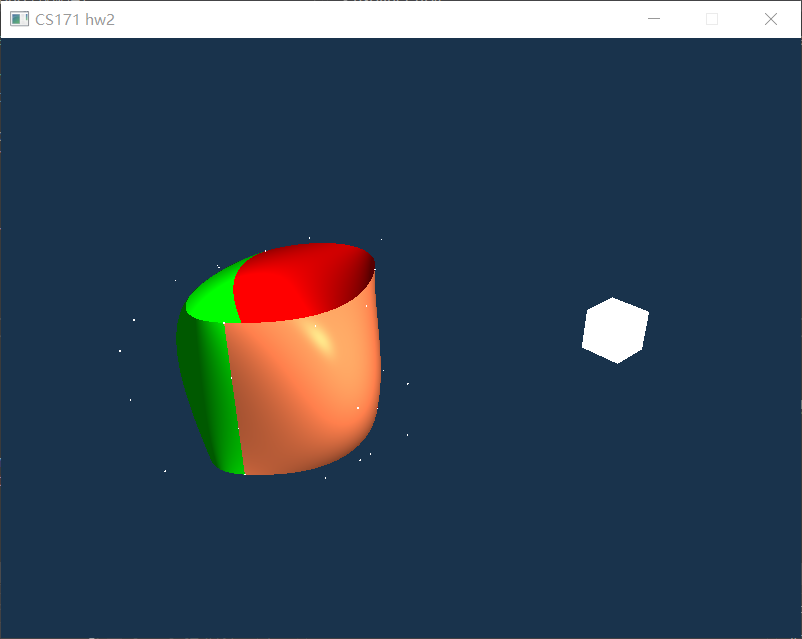
\includegraphics[scale=0.25]{beziersurface.png}
		\caption{beziersurface front}
	\end{minipage}
	\\
	\begin{minipage}[b]{.4\linewidth}
		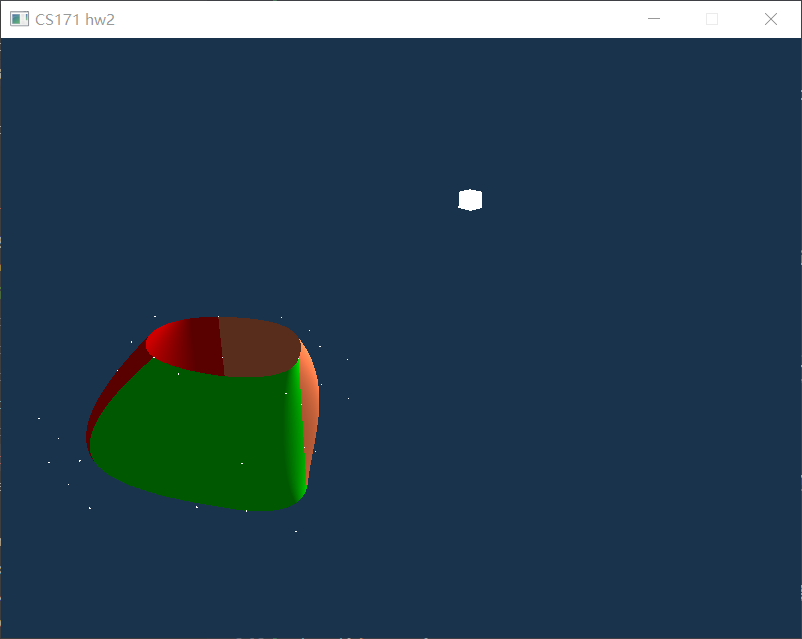
\includegraphics[scale=0.25]{beziersurface2.png}
		\caption{beziersurface back}
	\end{minipage}
	\\
	\begin{minipage}[b]{.4\linewidth}
		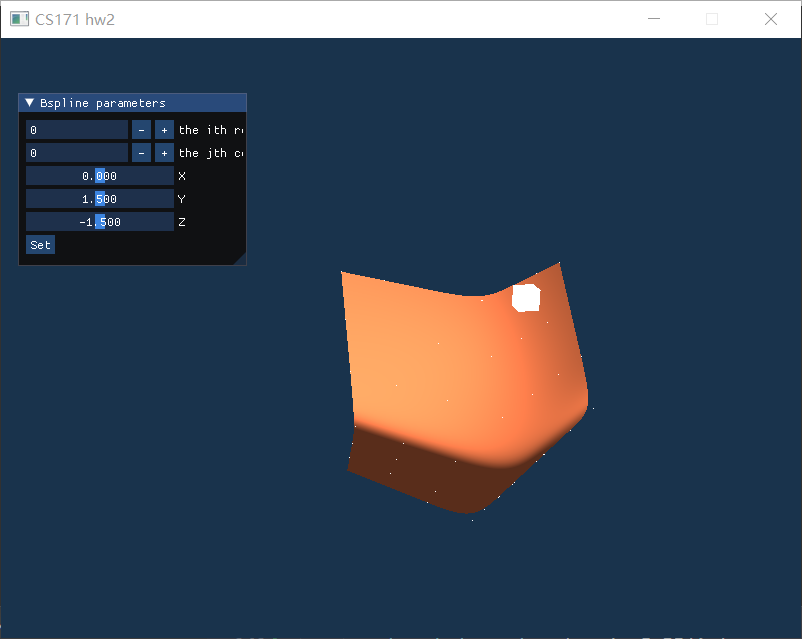
\includegraphics[scale=0.25]{bsplinesurface.png}
		\caption{bsplinesurface front}
	\end{minipage}
	\\
	\begin{minipage}[b]{.4\linewidth}
		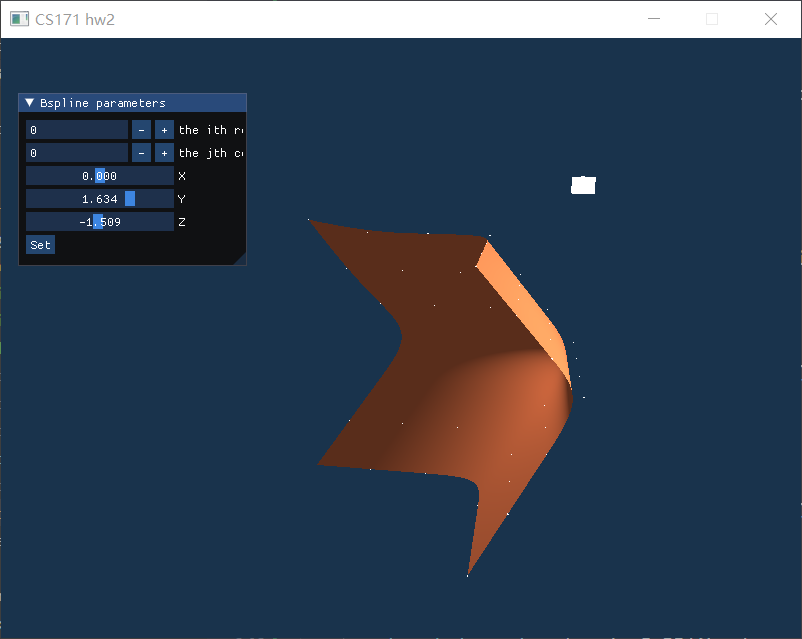
\includegraphics[scale=0.25]{bsplinesurface2.png}
		\caption{bsplinesurface back}
	\end{minipage}
\end{figure}


\end{document}

